%%&program=xelatex
%&encoding=UTF-8 Unicode
% SVN keywords
% $Author$
% $Date$
% $Revision$
% $URL$
\documentclass[a4paper,12pt]{article}  % Comments after  % are ignored
%\usepackage{hyperref}                 % For creating hyperlinks in cross references
%
\usepackage{ifxetex}% for XELATEX, or PDFlatex
\usepackage{ifplatform} 
%\usepackage{hyperref}
%\hypersetup{colorlinks=false}
%
\ifxetex
	\usepackage{polyglossia} \setmainlanguage{portuges}
	\usepackage{fontspec}
	\ifwindows
		\setmainfont[Ligatures=TeX]{Garamond}
		\setsansfont[Ligatures=TeX]{Gill Sans MT}
		\setmonofont{Consolas}
%		\setmonofont[Scale=MatchLowercase]{Courier}
	\fi
	\iflinux
		\setmainfont[Ligatures=TeX]{Linux Libertine O}
		\setsansfont[Ligatures=TeX,Scale=MatchLowercase]{Linux Biolinum}
		\setmonofont[Scale=MatchLowercase]{Courier}
	\fi
	\ifmacosx
	% add settings
	% Use xelatex -no-shell ...
	\fi
	\usepackage{xcolor,graphicx} 
\else
	\usepackage[portuguese]{babel}
	%\usepackage[latin1]{inputenc}
	\usepackage[utf8]{inputenc}
	\usepackage[T1]{fontenc}
	\usepackage{graphics}                 % Packages to allow inclusion of graphics
	\usepackage{color}                    % For creating coloured text and background
\fi

\usepackage{enumitem}
\setlist{nolistsep}

\usepackage{amsmath,amssymb,amsfonts} % Typical maths resource packages
\usepackage[retainorgcmds]{IEEEtrantools}
\usepackage{caption}

\usepackage{tikz}
\usetikzlibrary{calc,arrows,decorations.pathmorphing,intersections}
\usepackage[font={small,sf},labelfont={bf},labelsep=endash]{caption}
\usepackage{sansmath}

%use as the last command into the preamble 
\usepackage[bookmarks,colorlinks]{hyperref}

\oddsidemargin 0cm
\evensidemargin 0cm

\pagestyle{myheadings}         % Option to put page headers
                               % Needed \documentclass[a4paper,twoside]{article}
\markboth{{\small \it  Laboratório de Física Experimental Básica}}
{{\small\it MEFT - 1º Sem. 2015/2016} }

\addtolength{\hoffset}{-0.5cm}
\addtolength{\textwidth}{2.5cm}
\addtolength{\topmargin}{-1.5cm}
\addtolength{\textheight}{3cm}

%\textwidth 15.5cm
%\topmargin -1.5cm
\setlength{\parindent}{0pt}
\setlength{\parskip}{1ex  plus  0.5ex  minus  0.2ex}
\parindent 0.5cm
%\textheight 25cm
%\parskip 1mm


% Math macros
\newcommand{\ud}{\,\mathrm{d}} 
\newcommand{\HRule}{\rule{\linewidth}{0.5mm}}

\author{Prof. Bernardo B. Carvalho} 

%%%%, Bernardo Brotas Carvalho\\bernardo.carvalho@tecnico.ulisboa.pt} 
\date{ Setembro  2015} 

\begin{document} 

	
\includegraphics[width=0.2\textwidth]{../logo-ist}%\\[1cm]  %%  Logo_IST_color

	\HRule \\[0.5cm]
	{ \huge \sf  \textsc{Efeito fotoeléctrico}} \\[0.4cm] % \bfseries 
%	{ \huge \sf  \textsc{Construções Geométricas em Lentes Delgadas (aproximação paraxial)} }\\[0.4cm] % \bfseries 
	{ \large \bfseries Determinação da constante de Planck.}\\
%	{ \large \bfseries Procedimento Experimental}\\
	\HRule \\%[0.5cm]

\section{\sf OBJECTIVO DO TRABALHO}
\begin{itemize}
\item Verificação experimental do efeito fotoeléctrico.
\item Determinação da energia cinética dos fotoelectrões em função da frequência da luz incidente sobre a célula fotoeléctrica.
\item  Determinação da constante de Planck $h$.
%\item  Verificação da não-dependência da energia cinética dos fotoelectrões na intensidade da luz incdente na celula fotoeléctrica.
\end{itemize}


\section{\sf INTRODUÇÃO }
%\section{\sf }
%\subsection{\sf }
%\subsection{\sf Corpo esférico em queda livre num fluido}
O efeito fotoeléctrico era já conhecido no final do séc. XIX, com a emissão  de partículas carregadas da superfície de um metal quando iluminadas por luz intensa. Verificou-se também que a energia destas partículas, que mais tarde foram identificadas por eletrões, não dependia da intensidade da luz incidente mas sim do  seu comprimento de onda, $\lambda$.  A explicação correcta do efeito fotoeléctrico foi proposta em 1905 por Einstein\footnote{Pela qual recebeu o prémio Nobel em 1921.} baseada na teoria de Max Planck\footnote{Teoria Quântica da luz, pela qual recebeu o prémio Nobel em 1918.} da emissão-absorção da luz. Para ambos, a luz seria formada pela emissão de  corpúsculos (quantuns), que se batizaram como \emph{fotões}, cada um com energia $E$  dada por:

\begin{equation}
	\label{eq:energia2}
	E = h \nu %= K_e^{max} + W_O
\end{equation}
em que $h$ é apropriadamente a \emph{constante de Planck} e $\nu$ a frequência da luz ($\nu=c/\lambda$).  
%Em que $K_e^{max}$ é a energia cinética máxima dos fotoeletrões  e $W_O$ é a energia necessária para remover os eletrões da superfície do material ). 

De acordo com esta teoria corpuscular da luz, quando um fotão incide sobre a superfície de um metal é absorvido por um átomo, e a sua energia é depositada num dos electrões de valência.
% A estes electrões tem de ser depositada uma energia para que se libertem da rede metálica. 
 Se o fotão incidente tiver mais energia que um dado limiar ($W_O$ - \emph{Work function}, característica de cada metal), o  electrão é libertado da rede metálica e emitido do sólido com uma energia cinética $K_e = h\nu - W_O$.
A intensidade da luz determina assim o \emph{número de fotolectrões} emitidos, mas não a sua energia!

A figura \ref{fig:EFE}   representa esquematicamente o fotão incidente, a superfície do sólido, e os níveis de energia dos electrões de valência do material. Note que se a energia do fotão incidente não for suficiente (i.e. se $E_f < W_O$) não há emissão de fotoelectrões.

 
\begin{figure}[htb]   
\begin{center}
  \sansmath
    \begin{tikzpicture}[scale=0.25]
    \begin{scope} % Energy levels
        \draw (1,0) node[left] {$1s$} -- 
            ++(14,0) node[right] {$K$};
        \draw (1,4) node[left] {$2s$} -- 
            ++(14,0) node[right] {$L_1$};
        \draw (1,6) node[left] {$2p$} -- 
            ++(14,0) node[right] {$L_2,L_3$};
        \draw (0,12) -- 
            ++(16,0) node[right] {Nível  de Fermi};
        \draw[line width=0.9mm, black!50!white] (0,18) -- 
            ++(20,0) node[right] {Superfície};
    \end{scope}
    \begin{scope} % Valence and conduction bands
%        \draw (-8,7) rectangle node {banda de valência} 
%            ++(14,4);
        \draw (-8,13) rectangle node {banda de condução} 
            ++(14,4);
    \end{scope}
    \begin{scope} % Electrons
        \foreach \x in {3,5,...,11}
            \filldraw (\x, 6) circle (.75);
        \draw (11, 6) circle (.75);
        \foreach \x in {7, 9}
            \filldraw (\x, 4) circle (.75);
        \foreach \x in {7, 9}
            \filldraw (\x, 0) circle (.75);
        %\filldraw (7,0) circle (.75);
        
        %\filldraw(9, 0) circle (.75);
        
    \end{scope} 
    \begin{scope}[color=blue] % X-rays in, electron out
        \draw[decorate, decoration=snake] (12,20) 
            node[above] {$h\nu_b$}  -- (7,5.75);
        \draw[->] (7,5.75) -- (1,20);
        \filldraw (0.4,22) circle (0.75) node[right=5] {fotoeletrão};
    \end{scope}
    \draw[color=green,decorate, decoration=snake] (15,20) 
     node[above] {$h\nu_g$}  -- (9,5.75);

    \begin{scope}[color=red] % X-rays in, electron out
        \draw[decorate, decoration=snake] (18,20) 
            node[above] {$h\nu_r$}
            -- (9,0.75);
        %\draw[->] (9,0.75) -- (1,20);
        %\filldraw (0.4,22) circle (0.75) node[right=5] {fotoeletrão};
    \end{scope}
        
    \end{tikzpicture}

	\caption{Efeito fotoeléctrico}
	 \label{fig:EFE} 
	\end{center}
\end{figure}
	  
%\section{\sf Princípio do método}

A constante de Planck pode ser determinada expondo a superfície de um metal a luz monocromática, caracterizada por um comprimento de onda $\lambda=c /\nu$ fixo e medindo a energia cinética máxima dos fotoelectrões emitidos. A fig.~\ref{fig:plack_exp} representa esquematicamente uma montagem experimental para a realização desta experiência.

\begin{figure}[htb] 
	\centering 
	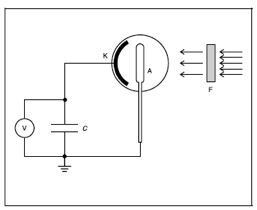
\includegraphics[width=0.6\textwidth]{planck_exp} 
	\caption{Diagrama esquemático da experiência do efeito fotoeléctrico.} \label{fig:plack_exp}
\end{figure}

%\begin{equation}
%	\label{eq:energia}
%	E= h \nu
%\end{equation}

A luz incide na superfície de um sólido metálico, designado \emph{cátodo} (K), através de um \emph{ânodo} (A) anelar ou transparente. 
Como cátodo é normalmente utilizado um metal alcalino (potássio, sódio ou cádmio)  pois neste caso os electrões de valência estão fracamente 
ligados ao núcleo (i.e. têm uma baixa função trabalho $W$ ). Como ânodo utiliza-se por exemplo a platina (Pt). 
O ânodo recebe parte dos fotoelectrões emitidos dando origem a uma corrente $I_f$ no circuito exterior. 
Se aplicarmos um potencial eléctrico retardador $V$ entre o ânodo e o cátodo a fotocorrente decresce, pois os fotoelectrões terão de vencer uma barreira de potencial eletrostática $U=e V$, onde $e$ é a carga do electrão. 
Para uma dada tensão crítica $V_s$ (potencial de paragem), deixa de existir fotocorrente. 
%Neste caso, mesmo os electrões mais fracamente ligados e que assim têm as maiores energias cinéticas, são parados. 

%$I_f=C\frac{dq}{dt}$
Experimentalmente pode usar-se uma fonte de tensão externa para aplicar o potencial de paragem. Mais simplesmente, pode usar-se um condensador para acumular a carga ($q=C V$) transportada pela própria corrente dos fotoelectrões (Fig.~\ref{fig:plack_exp}), aumentando gradualmente a diferença de potencial $V$, até atingir $V_s$ quando corrente é  auto-eliminada. Mas neste caso é necessário utilizar um voltímetro de impedância de entrada muito elevada ($> 10\textrm{ M}\Omega$) ou um amplificador electrónico de instrumentação, que é o caso da nossa montagem experimental.
 Após medir o potencial de paragem, podemos assim escrever:\footnote{Na realidade a função de trabalho tem de ser corrigida pelo potencial de contacto entre os dois metais, $W=W_O - \phi$, o que naturalmente não é importante para a determinação da constante de proporcionalidade.}

%, onde $e$ é a carga do electrão) entre o ânodo e o cátodo,
\begin{equation}
	\label{eq:energia}
	e\,V_s= K_e^{max}= h \nu - W_O
\end{equation}

Medindo o potencial de paragem sucessivamente para luz incidente de várias frequências, podemos então fazer o gráfico de $V_s\; vs. \;\nu$. Este gráfico deverá aproximar-se de uma recta de declive $h/e$ e ordenada na origem  $-W/e$.


\begin{figure}[htb]   
\begin{center}
  \sansmath
    \begin{tikzpicture}[y=3cm, x=.01cm,font=\sffamily]
 	%axis
	\draw (0,0) -- coordinate (x axis mid) (800,0);
    \draw (0,0) -- coordinate (y axis mid) (0,1.7);
    	%ticks
    	\foreach \x in {0,100,...,800}
     		\draw (\x,1pt) -- (\x,-3pt)
			node[anchor=north] {\x};
    	\foreach \y in {0,0.5,1.,1.5}
     		\draw (1pt,\y) -- (-3pt,\y) 
     			node[anchor=east] {\y}; 
	%labels      
	\node[below=0.8cm] at (x axis mid) {$\nu$ [THz]};
	\node[rotate=90, above=0.8cm] at (y axis mid) {$V_s$ [V]};
	%linha
    \draw (360,0) -- (760,1.5) node[above] {$h/e$};
     %\filldraw (400,1) circle (0.75); %node[right=5] {fotoeletrão};
	 %Pontos
	 \draw plot[mark=*,only marks] file {hplot.data};

    \end{tikzpicture}

	\caption{Exemplo da determinação de $h$ pelo efeito fotoeléctrico}
	 \label{fig:hplot} 
	\end{center}
\end{figure}

A constante $h$ é uma das constantes físicas fundamentais que se conhecem com maior precisão.
% relativa ($u_r = 3.4\times 10^{-8}$). 
O valor padrão actual é de $h=6.62606889(23) \times 10^{-34}\,\textrm{J}\cdot \textrm{s}=4.135667516(91)\times 10^{-15}\,\textrm{eV}\cdot\textrm{s}$ (os  dígitos entre parênteses representam a incerteza com a mesma resolução dos dois últimos dígitos do valor). 

A contínua procura de um valor mais preciso não é apenas um  desafio intelectual da comunidade científica, pois
 terá um efeito  revolucionário na ciência da Metrologia e todas as suas aplicações: 
 Como $h$ se pode relacionar com o número de Avogadro  $N_A$, quando se conhecer com maior precisão\footnote{O dispositivo mais preciso é a balança de Watt, onde se espera chegar à precisão de $u_r \sim 1\times 10^{-11}$} será possível re-definir a unidade padrão de massa do Sistema Internacional. a partir de um único átomo de um elemento químico, válido e diretamente utilizável em todo o Universo. 
 O padrão oficial actual de massa (kg) é o último ``resistente''  do sistema MKS que é baseado num artefacto: um cilindro de platina-irídio guardado a "sete chaves" em Sèvres, nos arredores de Paris\footnote{Ver por exemplo o artigo da revista \href{http://www.economist.com/node/18007494}{Economist} http://www.economist.com/node/18007494}.   
 
\section{\sf Procedimento Experimental}

\begin{figure}[htb] 
	\centering 
	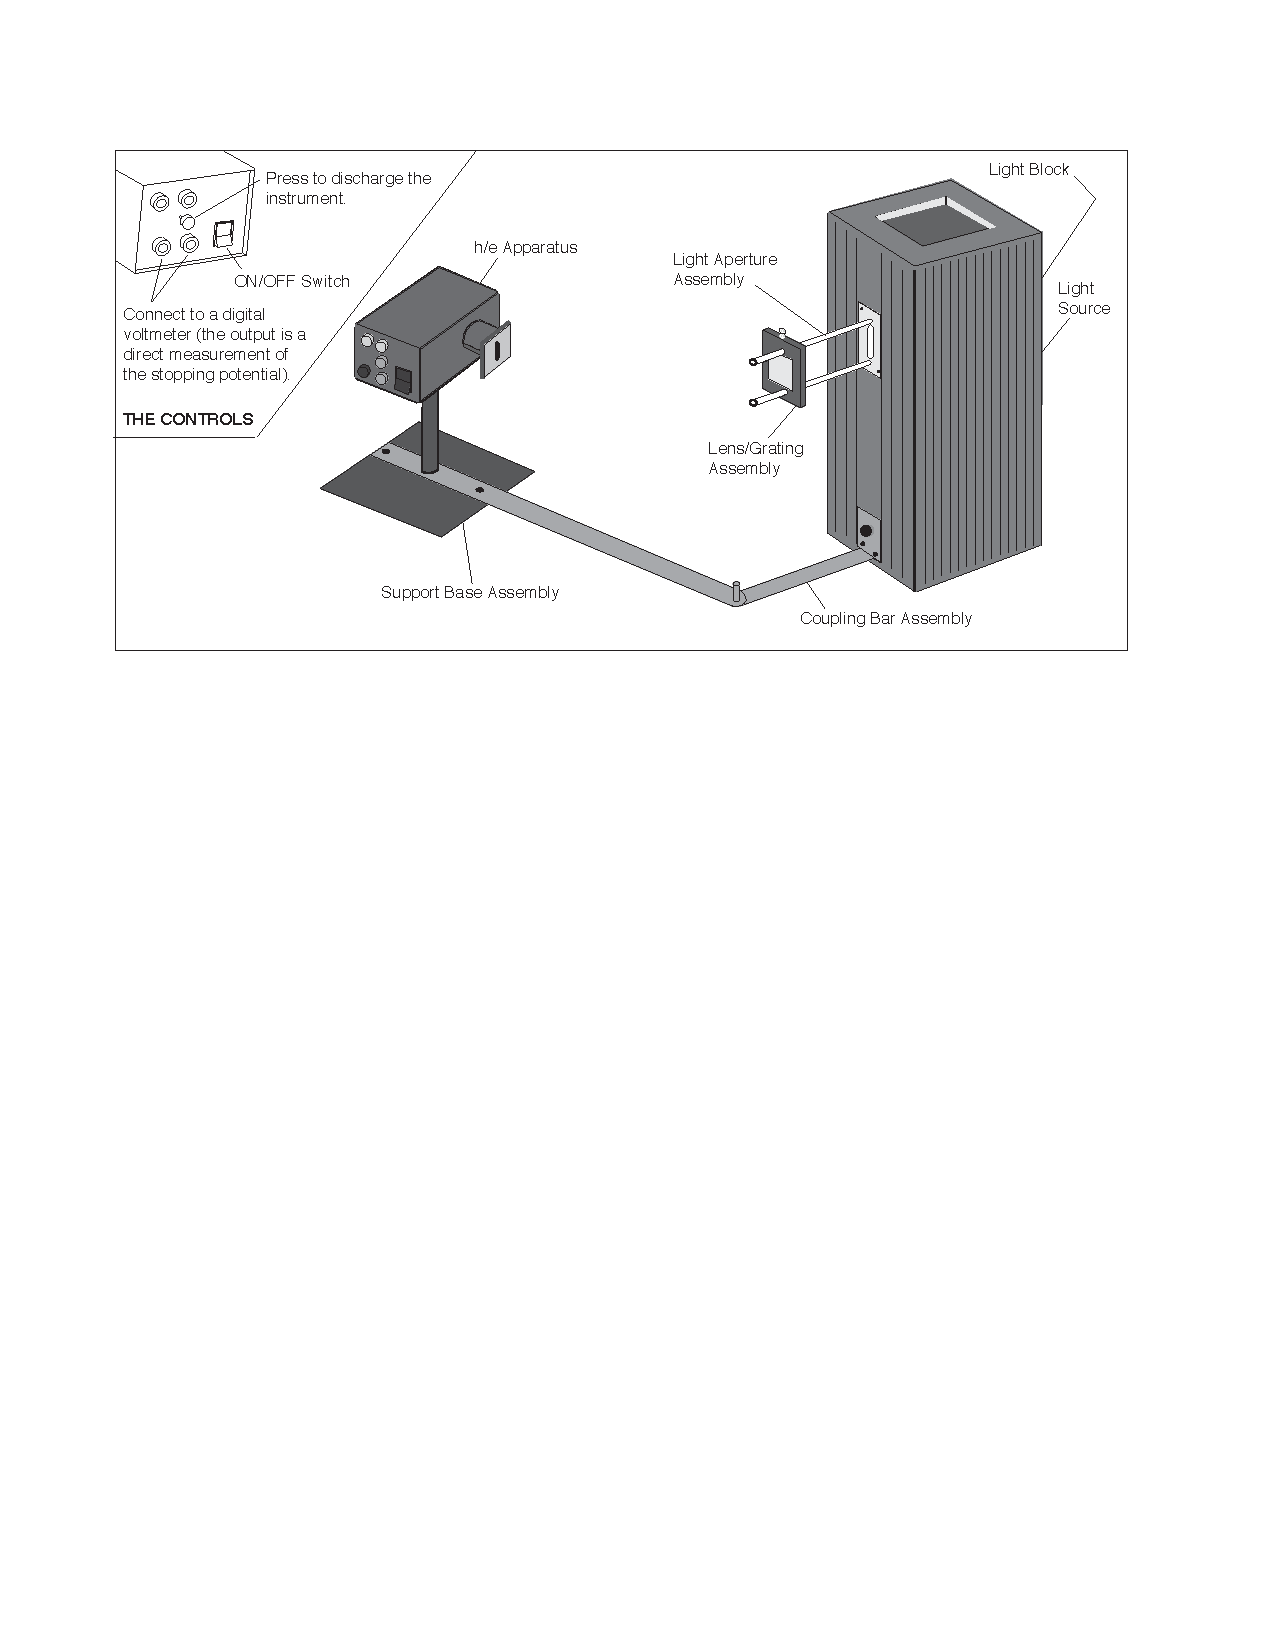
\includegraphics[width=0.8\textwidth]{planckPasco} 
	\caption{Montagem Experimental do efeito fotoelétrico} 
	\label{fig:plackPasco}
\end{figure}

\begin{enumerate}
\item Ligue a fonte de lâmpada de Mercúrio (Hg) e deixe estabilizar durante cerca de 10 min.
\item Enquanto espera, teste as tensões de cada uma das duas pilhas do amplificador da célula fotovoltaica.
\item Monte os componentes tal como indicado na Fig.~\ref{fig:plackPasco}.
\item Regule o conjunto de lente + rede de difração de modo a obter as riscas de cor bem focadas na zona do detector. Alinhe a montagem da fenda para que a célula esteja bem iluminada e centrada na risca.
\item O que observa depois da rede é uma \emph{figura de difracção}. 
%Observe as várias riscas, anote e interprete os ângulos de Difração e Ordem. 
Esta figura é simétrica (esquerda/direita) no que respeita às posições das riscas e das intensidades observadas? Quantas ordens de difracção consegue identificar?
\item Para cada uma das riscas (cores) pressione o botão de RESET e depois anote o valor da tensão de paragem e o tempo aproximado até a tensão estabilizar.
\item Repita o ponto anterior para outras duas riscas  e com pelo menos dois filtros de transmissão.
\end{enumerate}


\begin{table}[!hbp]
\begin{center}
	%\centering
	\begin{tabular}{|c|c|c|}
	\hline
	Cor  & Freq. [THz] & $\lambda$ [nm]  \\
	\hline
	Amarelo & 518.672 & 578 \\
	Verde & 548.996 & 546.074\\
	Azul & 687.858  & 435.835 \\
	Violeta & 740.858  & 404.656\\
	U.V.    & 820.264  & 365.483 \\
	\hline
 	\end{tabular}
	\caption{Riscas observáveis do espectro de Mercúrio.} 
	\label{tab:Hg}
	\end{center}
\end{table}

Pode consultar o espectro de Mercúrio em  \href{http://physics.nist.gov/asd}{
NIST Atomic Spectra Database}, esconhendo o elemento ``Hg I" e um \emph{Relative intensity minimum:} de $1000$, por exemplo. 	  	



%\newpage
%\section*{\sf Apêndice}



\end{document} 